%-----------------------------------------------------------------------------
%
%               Template for sigplanconf LaTeX Class
%
% Name:         sigplanconf-template.tex
%
% Purpose:      A template for sigplanconf.cls, which is a LaTeX 2e class
%               file for SIGPLAN conference proceedings.
%
% Guide:        Refer to "Author's Guide to the ACM SIGPLAN Class,"
%               sigplanconf-guide.pdf
%
% Author:       Paul C. Anagnostopoulos
%               Windfall Software
%               978 371-2316
%               paul@windfall.com
%
% Created:      15 February 2005
%
%-----------------------------------------------------------------------------


\documentclass[nocopyrightspace, 10pt]{sigplanconf}

% The following \documentclass options may be useful:
%
% 10pt          To set in 10-point type instead of 9-point.
% 11pt          To set in 11-point type instead of 9-point.
% authoryear    To obtain author/year citation style instead of numeric.

\usepackage{natbib}
\usepackage{url}
\usepackage[squaren,thinqspace,binary]{SIunits}

\usepackage{hyperref}
\newcommand\fnurl[2]{%
  \href{#2}{#1}\footnote{\url{#2}}%
}
\usepackage{lmodern}
\let\fourth\relax               % Undefine a macro
\let\second\relax               % Undefine a macro
\let\degree\relax               % Undefine a macro
\let\cdot\relax                 % Undefine a macro
\usepackage{array}
\usepackage{amsmath}
\usepackage{amssymb}
%\usepackage{mathabx}
\usepackage{mathtools}
\usepackage{multirow}
\usepackage{bussproofs}
\usepackage{verbatim}
\usepackage{fancyvrb}

\usepackage{graphicx}
\usepackage{subcaption,placeins}
\usepackage{setspace}
%\usepackage[tight,footnotesize]{subfigure}
% \usepackage{subfigure}

\usepackage{listings}
\usepackage{xcolor}

\usepackage{tabu}

% Display notes/comments with todonotes:
% \usepackage[disable]{todonotes} % notes/comments not showed
\usepackage[draft]{todonotes} % notes/comments showed


\usepackage{titlesec}
\usepackage{hyperref}

\titleclass{\subsubsubsection}{straight}[\subsection]

\newcounter{subsubsubsection}[subsubsection]
\renewcommand\thesubsubsubsection{\thesubsubsection.\arabic{subsubsubsection}}
\renewcommand\theparagraph{\thesubsubsubsection.\arabic{paragraph}} % optional; useful if paragraphs are to be numbered

\titleformat{\subsubsubsection}{\normalfont\normalsize\bfseries}{\thesubsubsubsection}{1em}{}
\titlespacing*{\subsubsubsection}{0pt}{1.25ex plus 1ex minus .2ex}{1.5ex plus .2ex}

\makeatletter
\renewcommand\paragraph{\@startsection{paragraph}{5}{\z@}%
  {3.25ex \@plus1ex \@minus.2ex}%
  {-1em}%
  {\normalfont\normalsize\bfseries}}
\renewcommand\subparagraph{\@startsection{subparagraph}{6}{\parindent}%
  {3.25ex \@plus1ex \@minus .2ex}%
  {-1em}%
  {\normalfont\normalsize\bfseries}}
\def\toclevel@subsubsubsection{4}
\def\toclevel@paragraph{5}
\def\toclevel@paragraph{6}
\def\l@subsubsubsection{\@dottedtocline{4}{7em}{4em}}
\def\l@paragraph{\@dottedtocline{5}{10em}{5em}}
\def\l@subparagraph{\@dottedtocline{6}{14em}{6em}}
\makeatother

\setcounter{secnumdepth}{4}
\setcounter{tocdepth}{4}

\usepackage{color}

\definecolor{mygray}{rgb}{0.4,0.4,0.4}
\definecolor{mygreen}{rgb}{0,0.8,0.6}
\definecolor{myorange}{rgb}{1.0,0.4,0}

\lstset{language=C++,
       basicstyle=\ttfamily\scriptsize,
       keywordstyle=\color{blue}\ttfamily,
       stringstyle=\color{red}\ttfamily,
       commentstyle=\color{green}\ttfamily,
       numbers=left,
       numbersep=5pt,
       numberstyle=\tiny\color{mygray},
       breaklines=true
      }

\newcommand{\fix}[1]{\texttt{\small #1}}

\begin{document}

%\titlebanner{banner above paper title}        % These are ignored unless
%\preprintfooter{preprint}   % 'preprint' option specified.

\title{ZOne --- A Data Parallel Language and Runtime}
\subtitle{CS533: Parallel Computer Architectures Final Project}

\authorinfo{Abdul Dakkak \and Carl Pearson \and Li-Wen Chang}
           {University of Illinois at Urbana-Champaign}
           {\{dakkak, pearson, lchang20\}@illinois.edu}

\conferenceinfo{CONF 'yy}{Month d--d, 20yy, City, ST, Country} 
\copyrightyear{20yy} 
\copyrightdata{978-1-nnnn-nnnn-n/yy/mm} 
\doi{nnnnnnn.nnnnnnn}

\maketitle

%\category{CR-number}{subcategory}{third-level}

%\terms
%term1, term2

%\keywords
%keyword1, keyword2

\begin{abstract}
The proliferation of GPUs in compute-heavy tasks has begun to extend to
big-data analytics. This places more emphasis on a new GPU-programming
difficulty - getting data onto the GPU in a way that does not adversely impact
performance.

We present a novel asychronous runtime, ZOne, that builds on prior work by
providing a unified
view of disk, GPU, and GPU memory. The runtime maintains
data and compute dependencies to optimize the schedule of I/O and compute
overlap. This provides a simplified programming interface and can further
improve performance.

We also present a new high-level language and compiler. The compiler targets
our asynchronous runtime and demonstrates some optimizations that can be done
on high-level languages to achieve performant code. We demonstrate that 
combining the language and asynchronous runtime can improve performance over
CUDA code with basic data transfer management by up to 8x on a machine with an
Intel Core i7-2820 and Nvidia Fermi Quadro 5010M.

\end{abstract}

\section*{Motivation and Overview}
Hello from intro.tex
\cite{placeholder}


\section{Motivation}

\begin{figure}
  \centering
    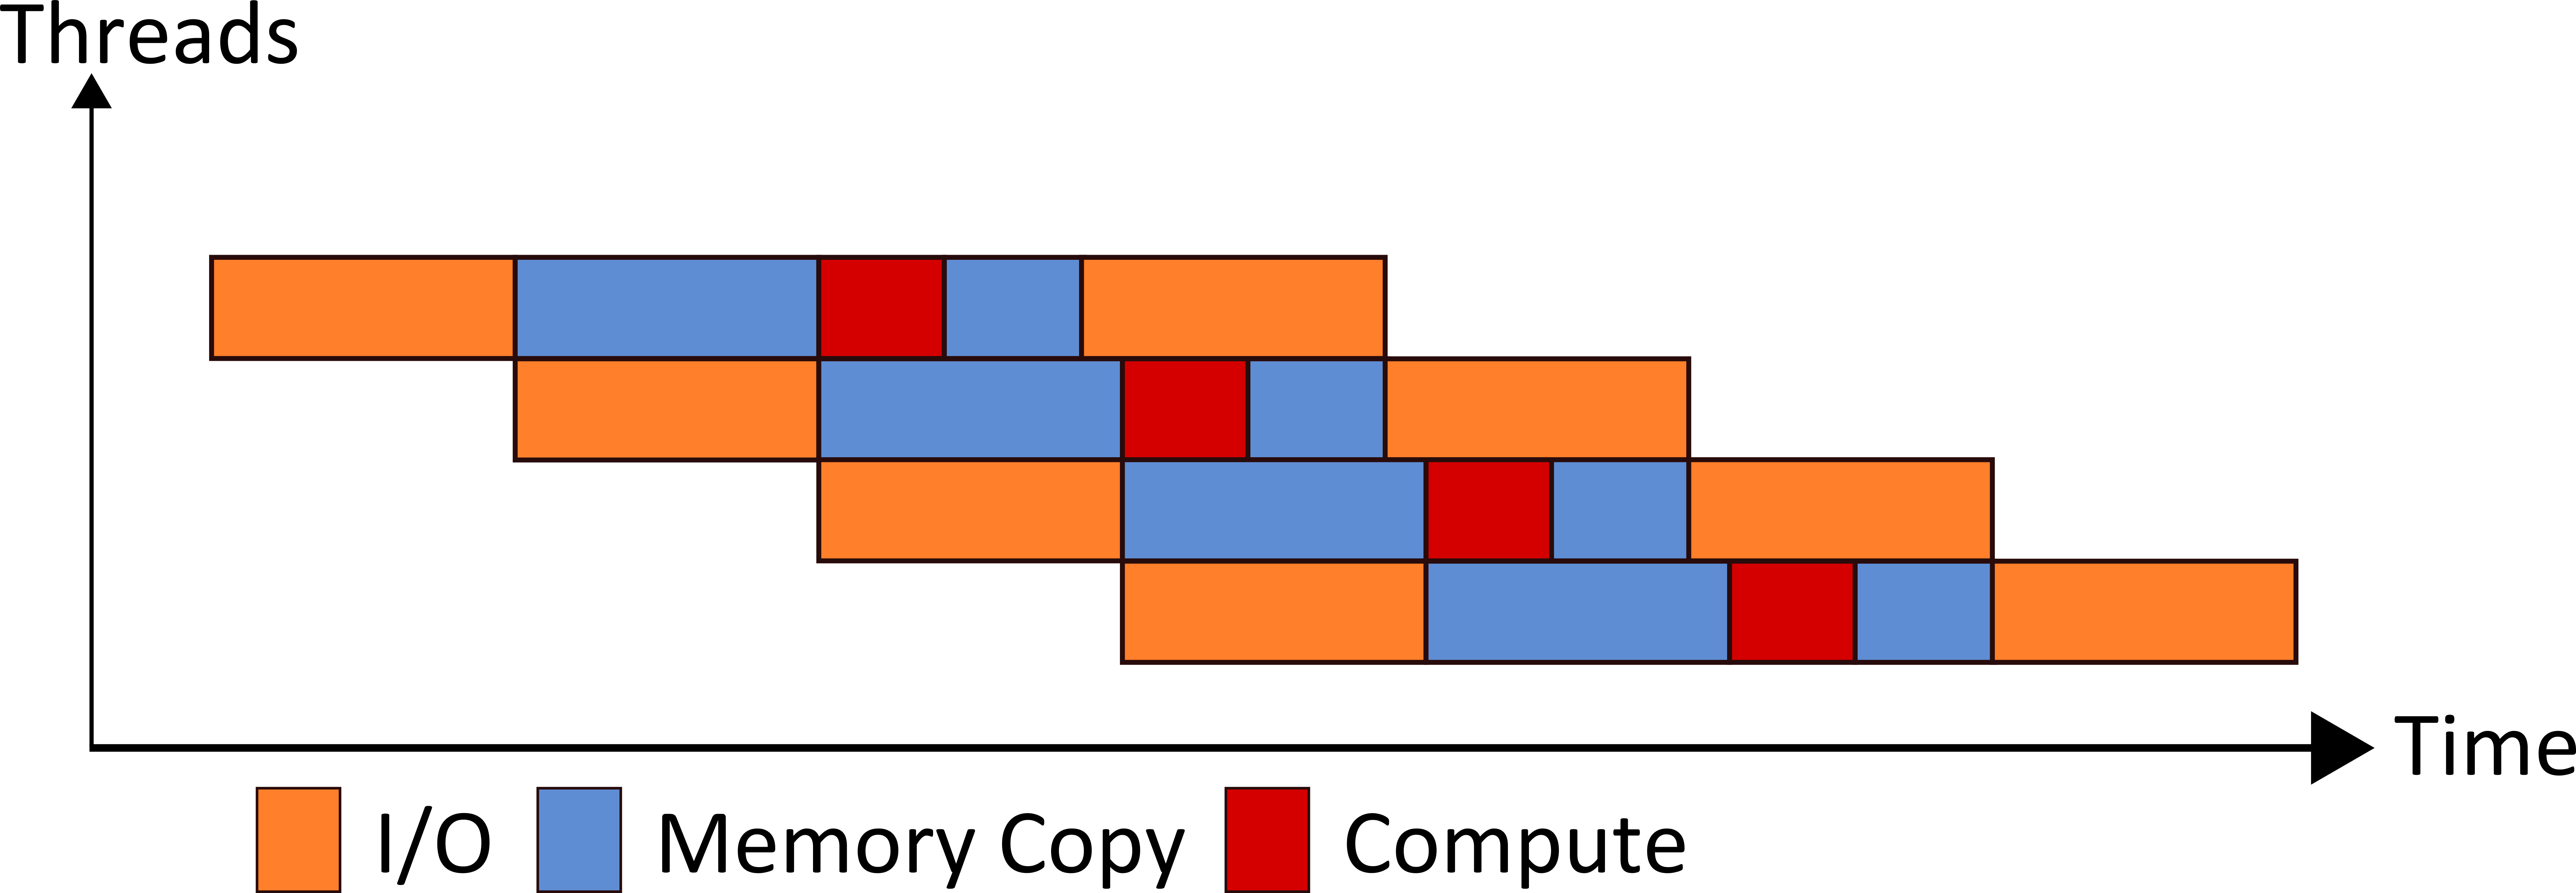
\includegraphics[width=0.5\textwidth]{fig/ord.png}
  \caption{A representation of simple overlap of host I/O, host-to-device data
           transfer, and kernel execution. In this example, there are no
           dependencies between kernels and data so management is relateively
           simple.}
  \label{fig:ord}
\end{figure}

\begin{figure}
  \centering
    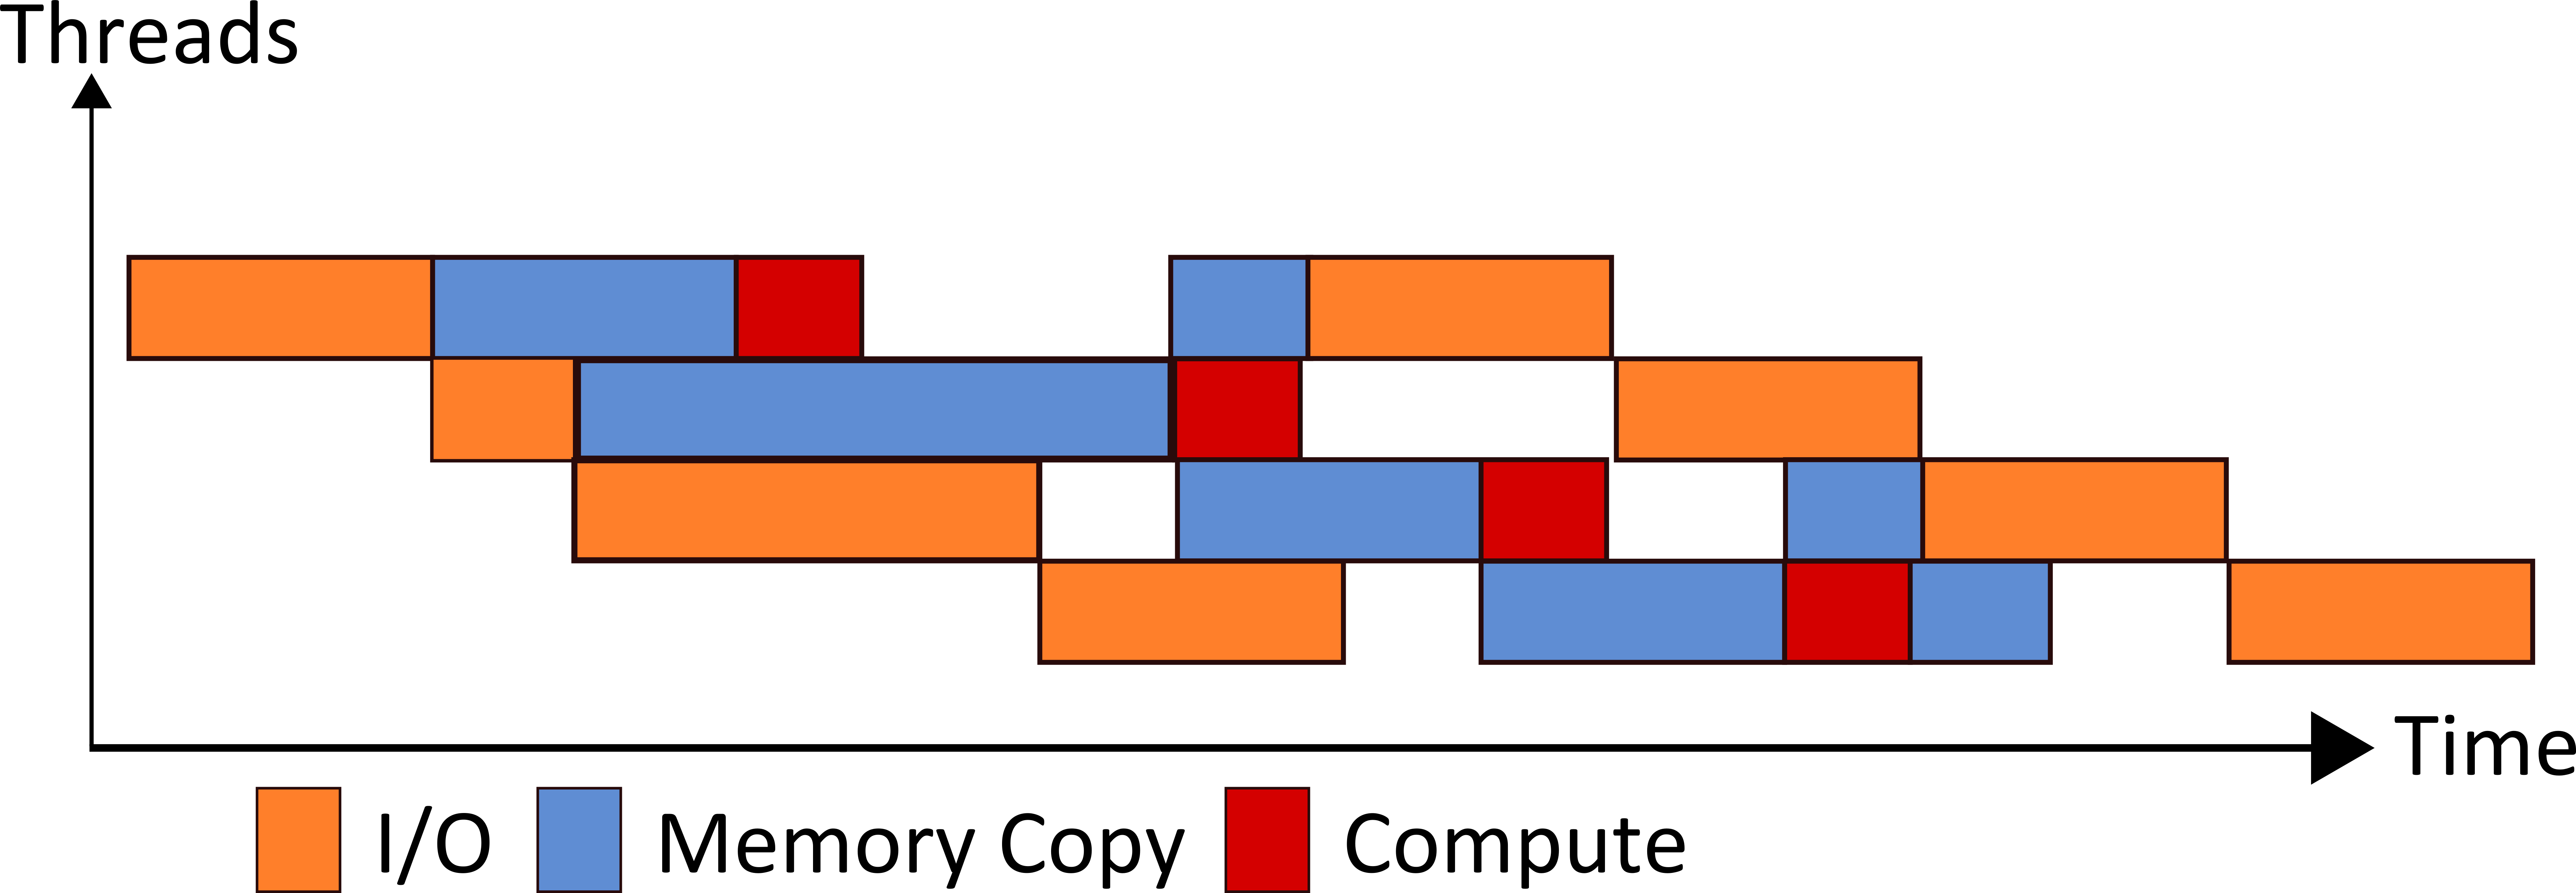
\includegraphics[width=0.5\textwidth]{fig/unord.png}
  \caption{A more complicated oververlap of host I/O, host-to-device data
           transfer, and kernel execution. Arbitrary data-dependence between
           kernels and transfers places too large a burden on the programmer
           to manage properly.}
  \label{fig:unord}
\end{figure}

When using GPUs to process big data, two major sources of latency are disk I/O
and data transfer between the host and device. OpenCL and CUDA provide methods
for managing simple patterns of overlap of data transfer and compute, shown in
Figure~\ref{fig:ord}. However, this does not assist with disk I/O.
Furthermore, in more complicated programs the existing methods are difficult to
implement efficiently. 

Figure~\ref{fig:unord} shows an example of overlapping in a more complicated
program varied I/O and transfer times. These dependencies are difficult to
efficiently manage statically because the latencies may not be known ahead of
time. Runtime management of these transfers is necessary to get efficient
results.

 


\section*{Implementation}

\subsection*{Overview}

ZOne currently targets CUDA code for NVIDIA GPUs.

\subsection*{Runtime}

\subsubsection*{CUDA Streams}
By design, CUDA device kernels execute asycnhronously with respect to the
host code. This allows host code to overlap with device code, but does not
allow different device operations (kernels and data transfers) to execute
concurrently. CUDA exposes device concurrency through \textit{CUDA Streams}
\cite{kirk2012programming}.

A CUDA Stream is a sequence of operations that
execute in-order on a CUDA device. Separate streams may be interleaved or
overlap if possible. In this way, it is possible to overlap computation and
memory transfers to hide the latency of some operations.
In order to effectively use streams, CUDA allows synchronization operations
to occur between arbitrary streams and provides host code that allows the
CPU to determine the execution status and progress of different streams.

The flexibility of CUDA streams is limited by the device hardware.
For example, the Fermi architecture can manage one queue of kernels, one queue
of device$\rightarrow$host transfers, and one queue of host$\rightarrow$device
transfers. Stream
dependencies between queues are maintained, but there are no dependencies
within queues - the operations are simply done in the order they are put into
the queue. This allows overlap of data transfer and compute on Fermi GPUs.
On devices that support more than one concurrent compute operation the amount
of concurrency is limited by the execution resources on the device. If both
operations are too large to run concurrently they will be serialized.
\subsubsection*{Intel Threaded Building Blocks}

\subsection*{Compiler Passes}


\section*{Evaluation}

\subsection*{Benchmarks}
To demonstrate the performance and correctness of our ZOne implementation, we
presently use three benchmarks: 2D convolution, histogram, and conjugate
gradient.

\subsubsection*{Convolution}
Convolutions have many uses in engineering and mathematics, particularly in
the image-processing fields. High-performance CPU convolution imlpementations
involve vectorization and tiling to make full use of cache bandwidth and 
execution resources. The ZOne convolution code is shown below

\begin{verbatim}
such code    wow

   impress
                speed
\end{verbatim}


\subsubsection*{Histogram}
Histograms are a fundamental analysis tool in image and data processing.
Efficient serial CPU histogram implementations are very straghtforward, but
due to the data-dependant access pattern efficient GPU implementations are
more involved. They typically feature privitization,
where individual histograms for portions of the data are computed separately
and then compiled together into the overall result. This reduces serialization
of atomic memory accesses when different threads increment the same bin.
Other approaches include sorting the input data and then finding the start
index of each bucket, and approaches that use graphics-specific hardware like
occlusion queries.

\begin{verbatim}
such code    wow

   impress
                speed
\end{verbatim}


\subsubsection*{Conjugate Gradient}

\begin{verbatim}
such code    wow

   impress
                speed
\end{verbatim}



\section{Prior Work}

As it pretains to prior work within the IMPACF group,
	the memory management is one that has some presidence.
Prior work was primarily concerned with either memory mamangemenet
	or hiding implementation details.

In~\cite{gmac} the authors hide CPU
	to GPU copy latency and unifying the 
	address space (from the programmer's point of view)
	of GPU and CPU devices.
Our work extends this by also managing file I/O and thus
	unifying disk, CPU, and GPU memory.

In Triolet\cite{rodrigues2014triolet}, a programming interface and system for
distributed-memory clusters was implemented. Triolet is able to handle
task decomposition, scheduling, and communication from the algorithmic skeleton description. Using algorithmic skeletons Triolet is able to capture parallel
computation patterns and abstract away the details of the implementation.
Triolet presents the programmer with higher-order functions through which
expressed parallelism is automatically distributed across a cluster.

While both projects were done in the IMPACT group, this work does
	not borry any code other than some discussions with senior memembers
	and understanding of some of the challenges to overcome.
In the next section we describe related work outside the IMPACT group.

\section{Related Work}

This work that is related to our project emphasizes expression of 
data-parallelism through higher-order functions and high-level languages. In
this section, we present a selection of related works.

DryadLINQ\cite{yu2008dryadlinq} is a high-level language for data-parallel
computing. It is designed to handle batch operations on large-scale
distributed systems. It combines strongly-typed .NET objects,
general-purpose declarative and imperative statements, and LINQ expressions
into a sequential program that can be debugged with a standard .NET debugger.
The DryadLINQ system automatically transforms the data-parallel portions of the
program into a distributed execution plan.
% TODO: more to write?

Triolet\cite{rodrigues2014triolet} is a programming interface and system for
distributed-memory clusters that handles task decomposition, scheduling, and
communication. Triolet emphasizes algorithmic skeletons to capture parallel
computation patterns and abstract away the details of the implementation.
Triolet presents the programmer with higher-order functions through which
expressed parallelism is automatically distributed across a cluster.

Thrust\cite{thrust} is a parallel algorithms library for C++ resembling the C++
standard library. Thrust code can use CUDA, Intel TBB, or OpenMP as a final
target to enable high performance across a variety of systems.

Copperhead\cite{copperhead} is a data-parallel version of a subset of Python
that is
interoperable with traditional Python code and Numpy. Copperhead can use CUDA,
Intel TBB, and OpenMP to accelerate operations. The Copperhead runtime
intercepts annotated function calls and transforms them (and their input data)
to the appropriate
CUDA, OpenMP, or TBB constructs before executing them.

Accelerate\cite{accelerate} is an embedded array language in Haskell for 
high-performance
computing. It allows computations on multi-dimensional arrays to be expressed
through collective higher-order operations such as maps or reductions. It has
a CUDA and OpenCL backend.

NOVA\cite{collins2013nova} is a data-parallel polymorphic, statically-typed
functional language. Parallelism is expressed through higher-order functions
such as scan, reduce, map, permute, gather, slice, and filter. NOVA has a
squential/parallel C backend, and a CUDA backend.

Adaptive Implementation Selection in SkePU\cite{enmyren2010skepu} is a C++ template library for data-parallel
computations on one or more GPUs through CUDA or OpenCL. SkePU programs are
expressed through skeletons derived from higher-order functions. Notably,
SkePU also implements lazy memory copying to avoid unecessary memory transfers.

GPU MapReduce (GPMR)\cite{stuart2011multi} is a  MapReduce library written
for multi-GPU clusters. GPMR programs are expressed through the map and reduce
higher-order functions. GPMR breaks these programs up into a map stage, a sort stage, and a reduce stage, then uses optimizations that reduce communication at
the expense of computation, which is a tradeoff that is well-suited for GPUs.
These optimizations are all based off of the data partitioning that the
programmer selects.

\section{Future Work}

While ZOne demonstrates some important features of an effective parallel
programming environment, there is plenty of opportunity to improve the
applicability and efficiency of the code generation.

\subsection{Runtime}

Support for OpenCL, a heterogeneous computing framework for writing programs
that run
on CPUs, GPUs, DSPs, FPGAs, and other available computing resources, would be a
logical step for the runtime. OpenCL is inspired by CUDA and has stream-like
capabilities, so many of the CUDA constructs that ZOne can
generate code for can easily be retargeted to OpenCL to allow ZOne to generate
efficient code for devices that are not NVIDIA GPUs. 

\subsection{Compiler}

It is worth mentioning that our aim was not to write an optimized
compiler (the compiler can be very slow), our aim was to have a compiler
that can generate optimized code. To that end, we have written the
compiler in Dart (a Javascript inspired language) that currently
generates sequential Javascript and threaded CUDA code from our language.
The Javascript
generation is primarily meant for debugging purposes.

\todo[inline]{finish}


% We recommend abbrvnat bibliography style.

\bibliographystyle{abbrvnat}
\bibliography{paper}

\listoftodos

\newpage


\section{Appendix}

\lstinputlisting[language=C++, label={lst:blackscholes}, caption=Black-Scholes using ZOne Runtime]{code/blackscholes.cu}

\end{document}
